%%%%%%%%%%%%%%%%%%%%%%%%%%%%%%%%%%%%
%              PROJECT             %
%%%%%%%%%%%%%%%%%%%%%%%%%%%%%%%%%%%%
\section{PROJECT}
\subsection{AZ Breast Cancer Detailer}
Environment: Veeva
GIT:  https://github.com/HealthyDigital/Projects\_2016.git 
Branch: dev

\subsection{Project structure}
The project consist of two presentation.The main presentation AZ Breast Cancer and the hidden reference presentation AZ Breast Cancer References (ID:AZANZBREF). For the main presentation the following folders are relevant:
\begin{lstlisting}[language=sh, caption=Presentation parts,label=lst:folders]
Intro
Zoladex
Nolvadex
common
\end{lstlisting}

All parts share common javascript, font, css and image files located under {{\textbackslash common\textbackslash OncologyBreastCommon}}. These files are linked into the assets of each part through a soft link "shared":

\begin{lstlisting}[language=sh, caption=Soft link,label=lst:softlink]
drwxr-xr-x  10 admin2-gesine  wheel     340  6 Sep 16:07 ..
drwxr-xr-x   7 admin2-gesine  wheel     238  4 Sep 17:52 .
-rw-r--r--@  1 admin2-gesine  wheel    8814  4 Sep 17:52 AZ-00-Intro-thumb.jpg
-rw-r--r--@  1 admin2-gesine  wheel  132571  4 Sep 17:51 AZ-00-Intro-full.jpg
-rwxr-xr-x   1 admin2-gesine  wheel    5236  4 Sep 12:08 AZ-00-Intro.html
lrwxr-xr-x   1 admin2-gesine  wheel      13  4 Sep 11:49 shared -> ../../common/
\end{lstlisting}

To build the assets into zips execute the createZips.sh script in the scripts folder of each part inside a terminal. The created new zip files can then be found in the zips folder. 

\begin{lstlisting}[language=sh, caption=Create asset zips,label=lst:createZips]
Admin2-Gesine:Intro admin2-gesine$ cd scripts/
Admin2-Gesine:scripts admin2-gesine$ ./createZips.sh 
\end{lstlisting}


%%%%%%%%%%%%%%%%%%%%%%%%%%%%%%%%%%%%
%          HEALTHY ENV             %
%%%%%%%%%%%%%%%%%%%%%%%%%%%%%%%%%%%%
\newcommand{\qq}{\symbol{34}} % 34 is the decimal ascii code for "
\newcommand{\FormatApiMethod}[1]{\bfseries{#1}}
\newcommand*{\FormatCell}[1]{\textcolor{lightgrey}{\MakeUppercase{#1}}}
\newcolumntype{U}{>{\collectcell\FormatCell}r<{\endcollectcell}}
\section{Healthy Sandbox Environment} 
Direct upload into test.salesforce.com as cloader

\begin{itemize}
\item AZ Breast Cancer (ID:AZAUBC)
\item shared resources: OncologyBreastCommon
\item AZ Oncology Breast References (ID:AZANZBREF)
\end{itemize}

\section{AZ C01 Sandbox Environment}
Upload through Vault PromoMats:https://login.veevavault.com (Dan.Davis@astrazeneca.com)\\
(Please don't migrate the presentation from our CRM to c01 it won't work!)

\begin{itemize}
\item AZ Breast Cancer\_1 (ID: AZAUBC1)
\item shared resources: OncologyBreastCommon
\item AZ Breast Cancer References (ID:AZANZBREF)

\end{itemize}

\subsection{Update process with PromoMats}
The process how to get an update of a presentation into C01 via PromoMats is depending on the current state of the binder (PromoMats version of a presentation).

\begin{center}
\begin{figure}[!h]
\centering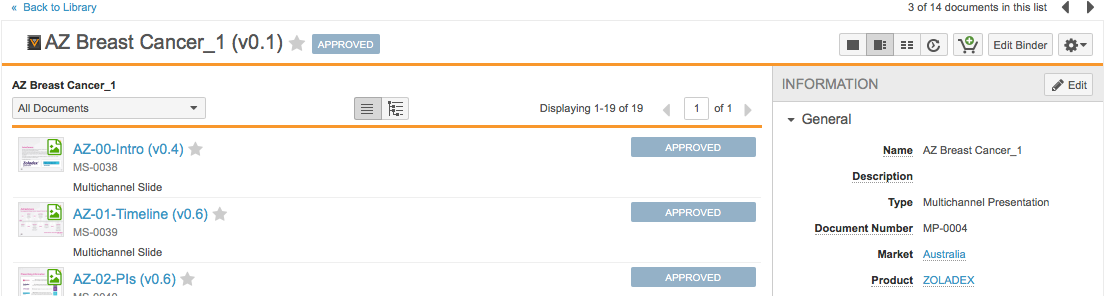
\includegraphics[width=\textwidth]{images/approved.png} 
\caption{Approved binder} \label{fig:approved}
\end{figure}
\end{center}
 

In case the presentation has been APPROVED and is therefore in production a new DRAFT version needs to be created for the binder and for each asset which has to be updated. 

\begin{center}
\begin{figure}[!h]
\centering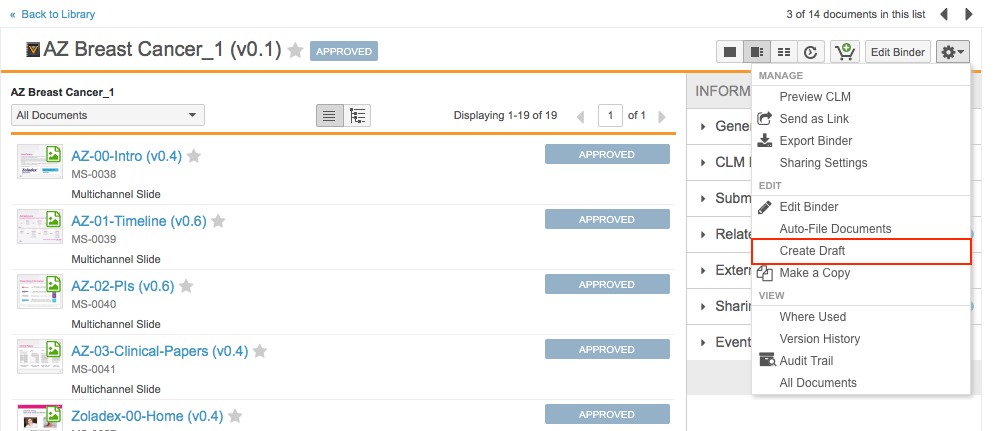
\includegraphics[width=\textwidth]{images/createDraftBinder.png} 
\caption{Create a new draft version of the binder} \label{fig:draftBinder}
\end{figure}
\end{center}

\begin{center}
\begin{figure}[!htb]
\centering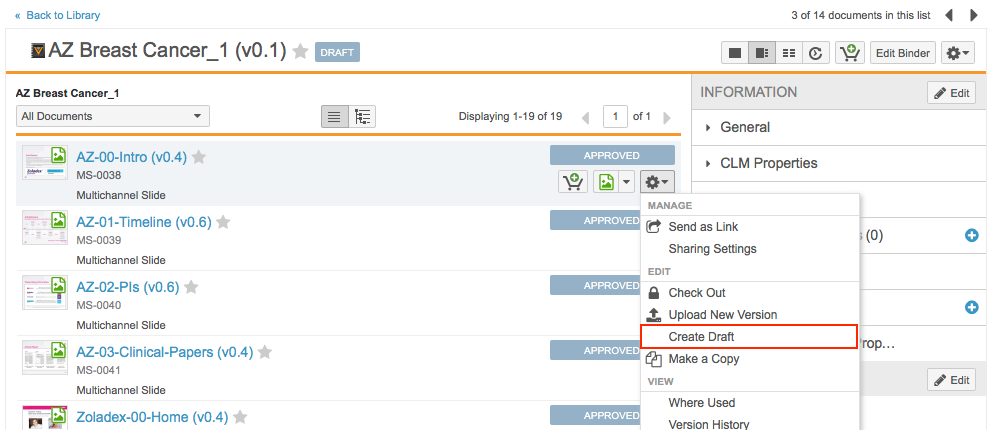
\includegraphics[width=\textwidth]{images/createDraftAsset.png} 
\caption{Create a new draft asset version} \label{fig:draftAsset}
\end{figure}
\end{center}

DRAFT versions are not visible in any environment. To make the changes visible in c01 the draft binder and draft assets need to be moved to staged. See fig:\ref{fig:moveAssetToStaged} In case the presentation and slides are already STAGED to update asset just upload a new version (see fig: \ref{fig:uploadNewVersion}).

\begin{center}
\begin{figure}[!htb]
\centering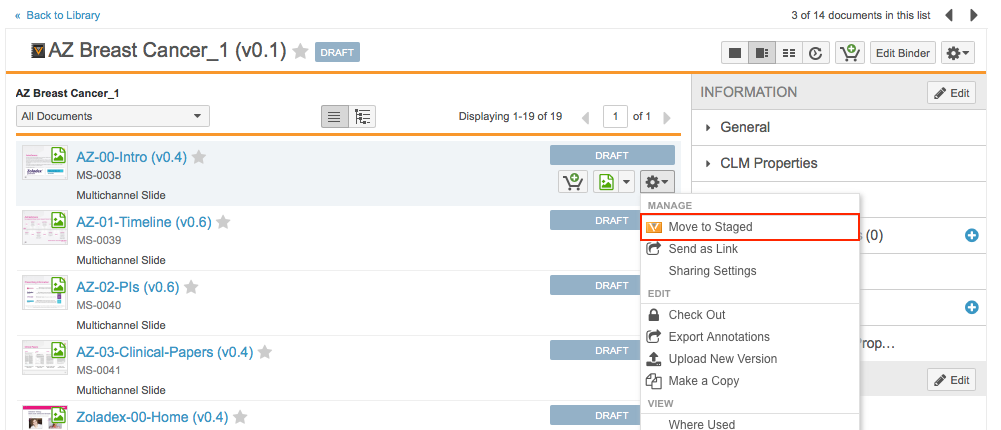
\includegraphics[width=\textwidth]{images/moveAssetToStaged.png} 
\caption{Move asset to staged} \label{fig:moveAssetToStaged}
\end{figure}
\end{center}



\begin{center}
\begin{figure}[!htb]
\centering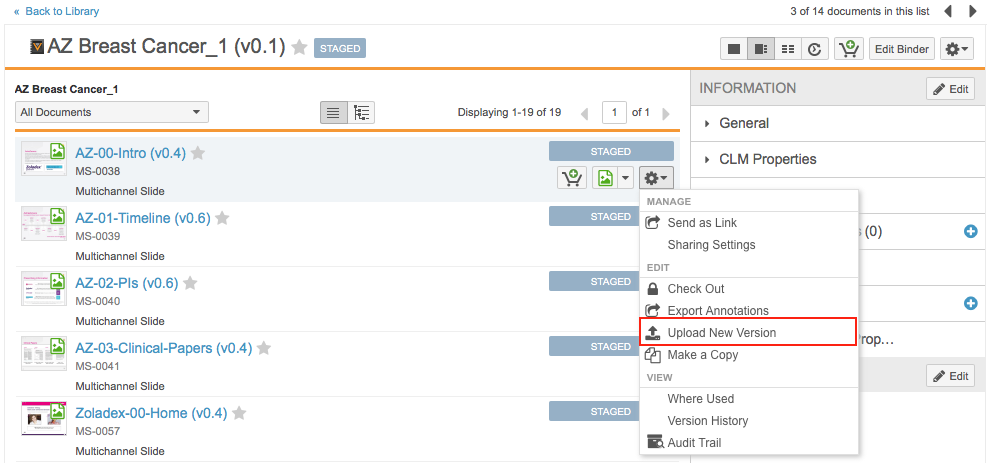
\includegraphics[width=\textwidth]{images/uploadNewVersion.png} 
\caption{Upload new version} \label{fig:uploadNewVersion}
\end{figure}
\end{center}

\subsection{CRM synchronisation}

When all changes are uploaded to Vault PromoMats and set to STAGED the CRM needs to synchronise the changes to make them available on the iPad. Therefore log into test.salesforce.com as bene@az.anz.c01 and go to "CLM Administration" (it's under the plus in the top level menu) and hit the "Sync" button next to "CLM Subscription History". If the synchronisation was successfull the status will be Finished (fig:\ref{fig:finished}) or Failed in case of an error (fig:\ref{fig:failed}). There will be a link to a csv file with some more or less helpful information which data has failed and why. 

\begin{center}
\begin{figure}[!htb]
\centering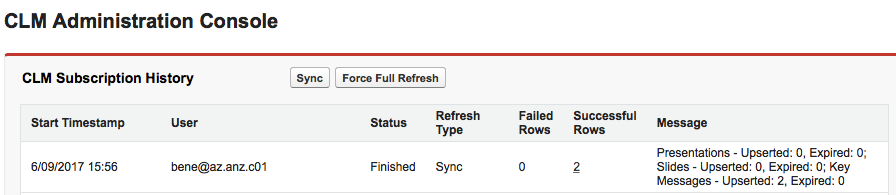
\includegraphics[width=\textwidth]{images/finished.png} 
\caption{Successfull synchronisation} \label{fig:finished}
\end{figure}
\end{center}

\begin{center}
\begin{figure}[!htb]
\centering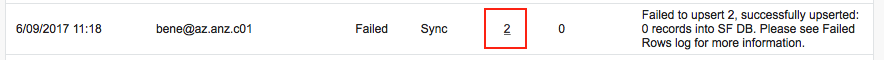
\includegraphics[width=\textwidth]{images/failed.png} 
\caption{Failed synchronisation} \label{fig:failed}
\end{figure}
\end{center}

\lstinputlisting[language=props,frame=tlrb,caption=Example Failed Data CSV,label=lst:faileddata]{listings/failed_history.csv}

\subsection{How to get the Vault PromoMats presentation into production}
To get the Vault PromoMats presentation into production Sharon needs to set all assets to APPROVED and synchronise the production system to make the changes available there. {{\bfseries IMPORTANT:}} the shared resource asset needs to be set to APPROVED as well. This needs to be done manually otherwise the presentation won't work in production because the latest shared css and javascripts are missing.